\section{useDirections}
Der Hook useDirections ist für die Google Maps Directions API-Anfragen zuständig. Google bietet über
ihre API die Möglichkeit an, die Distanz zwischen zwei Orten abzufragen, genau wie in Google Maps.

\begin{figure}[H]
  \begin{center}
    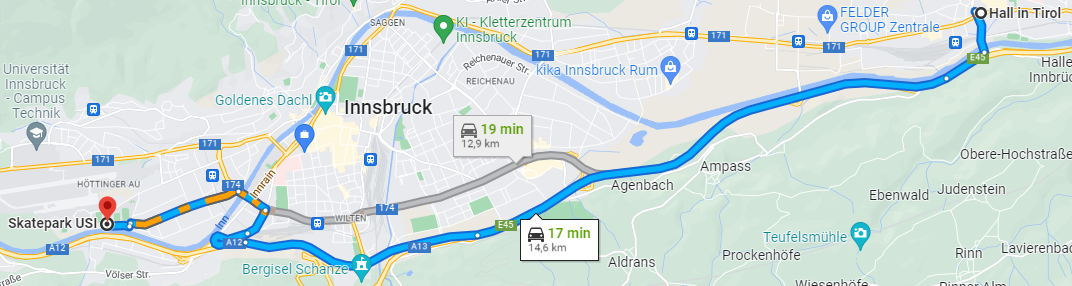
\includegraphics[width=0.5\textwidth]{Mobile/GoogleMapsDirections.png}
    \caption{Distanz zwischen Hall in Tirol und Skatepark USI Innsbruck}
  \end{center}
\end{figure}

\label{apikey}
Um diese API benutzen zu können benötigt man einen API-Schlüssel, welchen man unter
\url{https://console.cloud.google.com} erhält. Google ist mit ihrer Cloud Console einer der größten
Anbieter von Cloud Computing neben Amazon AWS und Microsoft Azure. Für diese Anfragen benötigt man
Zugriff auf die "Directions API".

\begin{lstlisting}
const buildUrl = method => {
  let url = 'https://maps.googleapis.com/maps/api/directions/json?origin=';
  url += location.coords.latitude.toString();
  url += ',';
  url += location.coords.longitude.toString();
  url += '&destination=';
  url += skatepark.latitude.toString();
  url += ',';
  url += skatepark.longitude.toString();
  url += '&mode=';
  url += method;
  url += '&key=';
  url += secrets.apiKey;
  return url;
};
\end{lstlisting}

Mit dieser Funktion bauen wir uns die URL für die Anfrage zusammen. Als Method übergibt man den
String "walking", "bicycling", "transit" oder "driving".